%=========================================================================
% (c) 2011, 2012 Josef Lusticky <xlusti00@stud.fit.vutbr.cz>

\section{Network and timestamps}\label{sec:ntp-network}
Network specification of NTP defines that
the protocol uses the User Datagram Protocol (UDP) on port number 123~\cite{ianna-ports,rfc5905}.
Reliable message delivery such as TCP can actually make the delivered of
NTP packet less reliable since retries
would increase the delay value and other errors~\cite{rfc5905}.
This is mostly due to overhead of communication with TCP on transport layer.

NTP manipulates with the time through timestamps - a record of time.
NTP timestamp has two fields: the seconds field expressing the number of seconds
and the fraction field expressing fraction of a second~\cite{rfc5905}.
All NTP time values are represented in twos-complement format, with
bits numbered in big-endian fashion from zero starting at the left, or high-order, position~\cite{rfc5905}. 
There are two formats of timestamp in NTP packet structure:
long 64-bit and short 32-bit as shown on figure~\ref{fig:ntp-timestamps}.
The 64-bit long timestamp used by NTP consists of a 32-bit unsigned seconds
field spanning $2^{32}$ seconds (approx. 136 years from 1900 to 2036) and a 32-bit fraction field resolving
$2^{-32}$ seconds (approx. 232 picoseconds)~\cite{rfc5905}.
The short 32-bit timestamp includes a 16-bit unsigned seconds field
and 16-bit fraction field.

Besides these two, there is one more NTP timestamp format - 128-bit NTP Date format.
It includes a 64-bit signed seconds field and 64-bit fraction field.
For convenience in mapping between formats,
the seconds field is divided into a 32-bit Era Number field
and a 32-bit Era Offset field.
This 128-bit NTP Date format is however not transmitted over the network
and is only used where sufficient storage and word size is available~\cite{rfc5905}.
There is practically no need of knowing about this format for embedded systems
at least until year 2036, when the Era Number will be incremented from zero to one.
But strictly speaking an NTP timestamp is a truncated NTP Date format~\cite{rfc5905}.
Refer to appendix~\ref{app:dates} for a short list of some dates
requiring usage of NTP Date format.

\begin{figure}
	\centering
	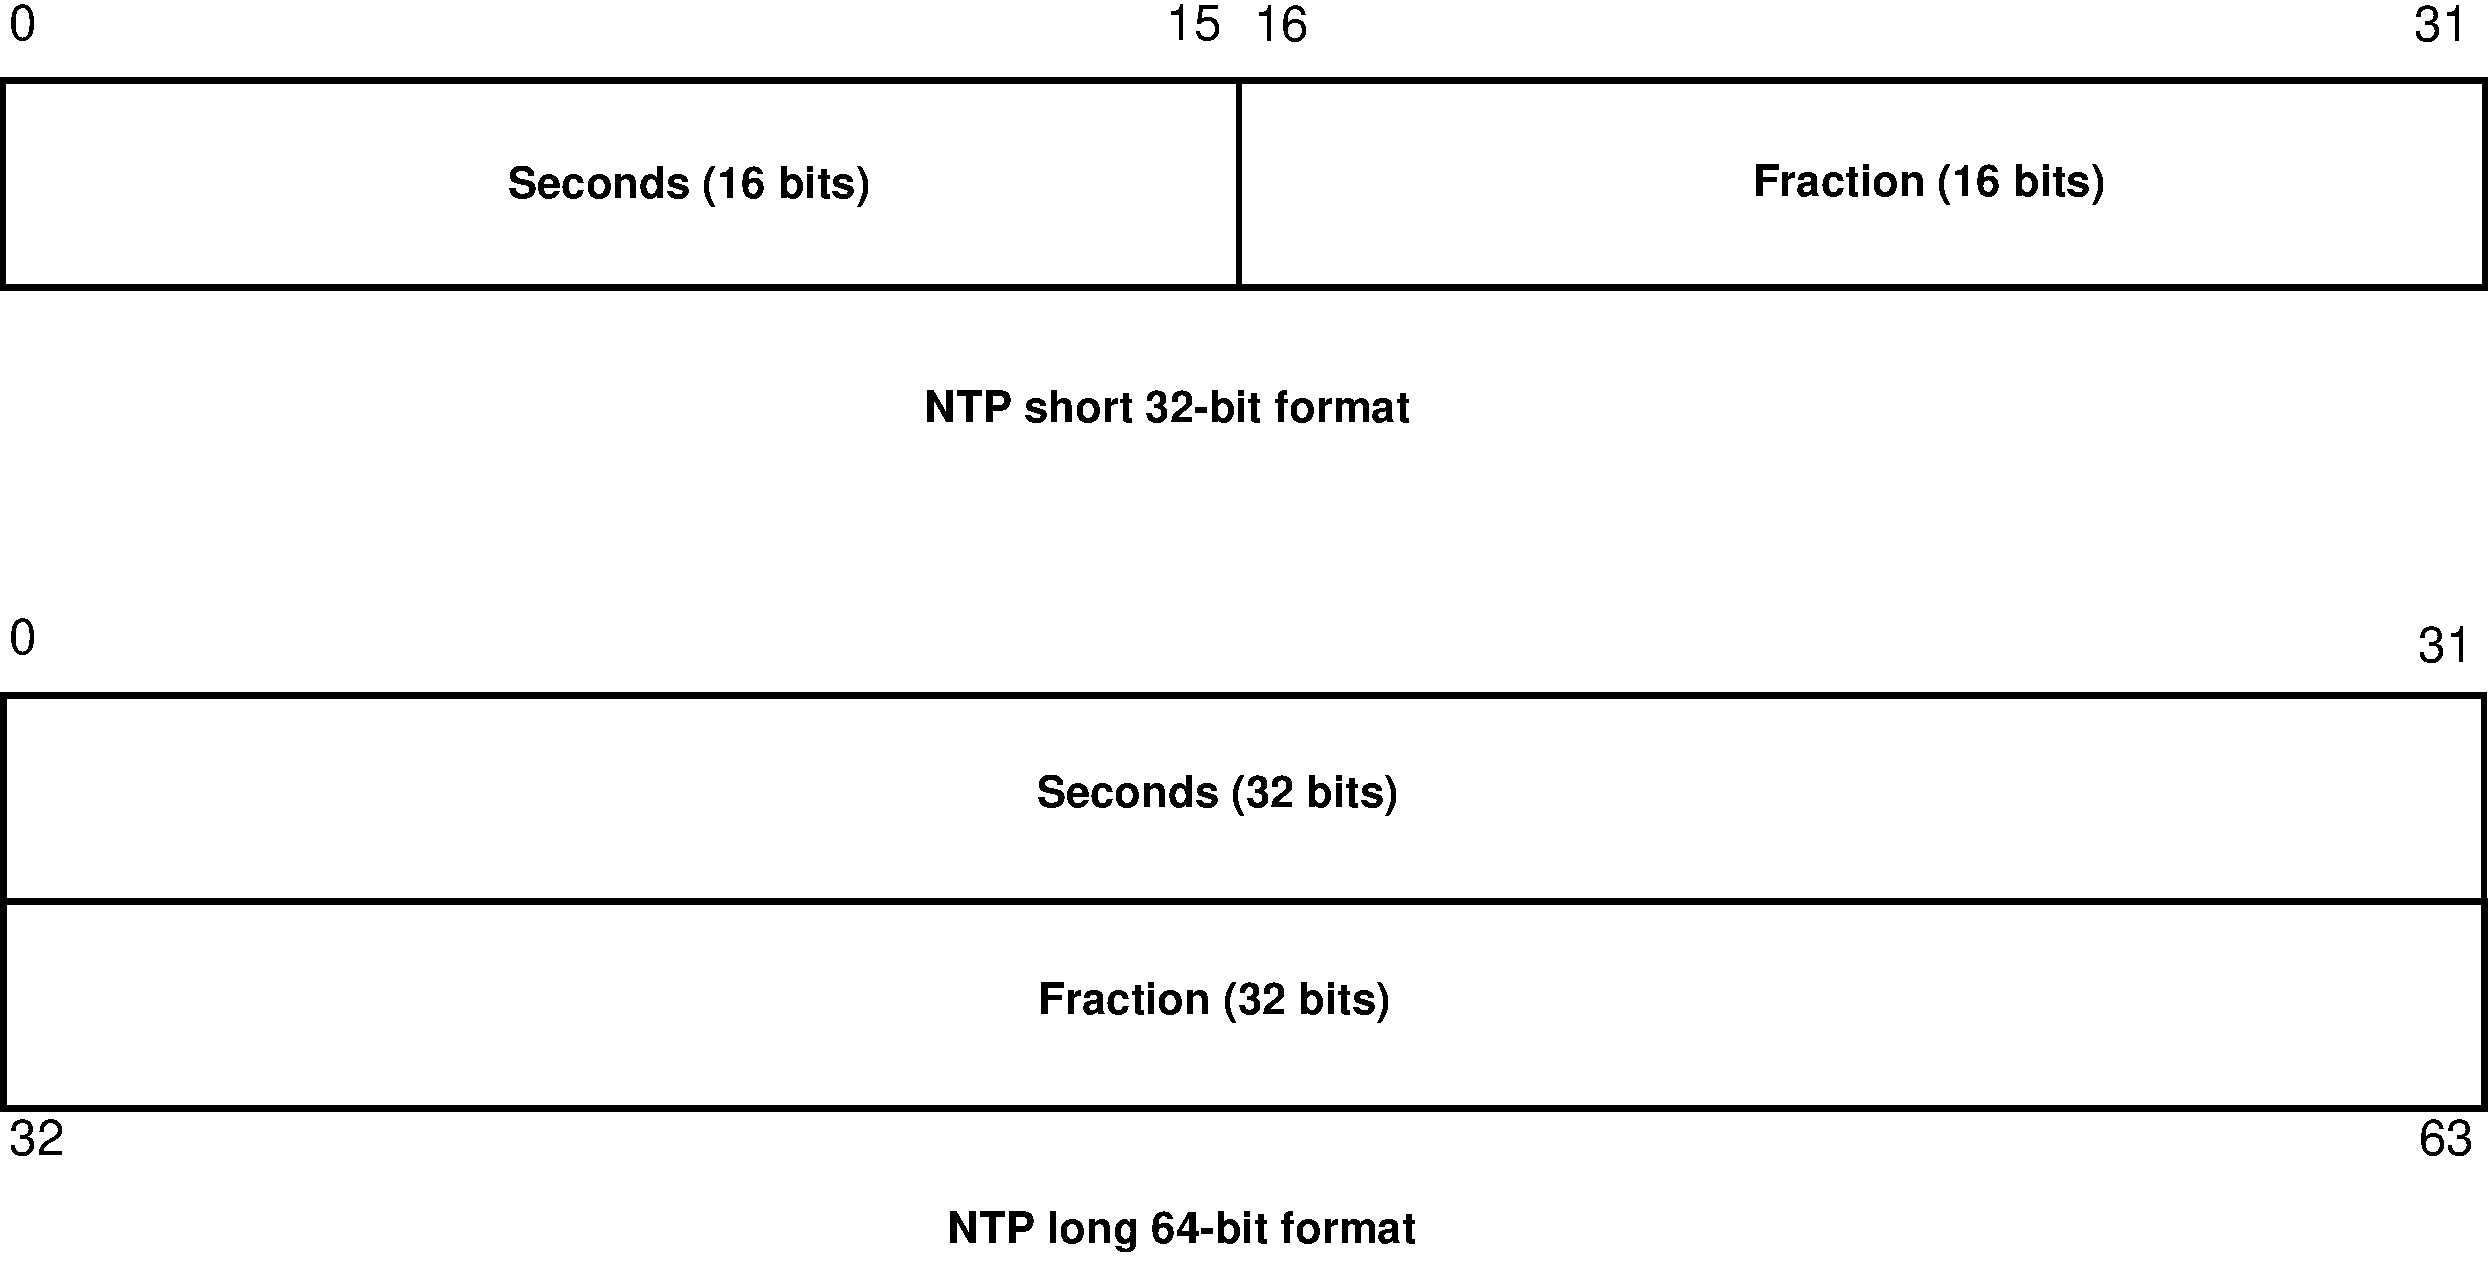
\includegraphics[width=13cm,keepaspectratio]{fig/ntp-timestamps.pdf}
	\caption{Time formats used in NTP packet}
	\label{fig:ntp-timestamps}
	\bigskip
\end{figure}

%! TODO
Standard NTP packet structure without Autokey extension is shown on figure~\ref{fig:ntp-packet}.

Leap Indicator (LI) is 2-bit integer warning of an impending leap
second to be inserted or deleted in the last minute of the current
month~\cite{rfc5905}.

Version Number (VN) is 3-bit integer representing the NTP
version number, currently 4.

Mode 3-bit integer representing the mode...
...In the unsymmetric mode the
      client periodically sends an NTP message to the server, which then
      responds within some interval.  Usually, the server simply
      interchanges addresses and ports, fills in the required
      information and sends the message right back. Servers operating in
      the unsymmetric mode then need retain no state information between
      client requests.
% BROADCAST MODE - rfc1769

Stratum is 8-bit integer representing the stratum.

7.4.  The Kiss-o'-Death Packet

   If the Stratum field is 0, which implies unspecified or invalid, the
   Reference Identifier field can be used to convey messages useful for
   status reporting and access control.  These are called Kiss-o'-Death
   (KoD) packets and the ASCII messages they convey are called kiss
   codes. 

Poll is 8-bit signed integer representing the maximum interval between
successive messages, in log2 seconds.
Suggested default limits for minimum and maximum poll intervals are 6 and 10, respectively.

Precision is 8-bit signed integer representing the precision of the
system clock, in log2 seconds.
For instance, a value of -18
corresponds to a precision of about one microsecond. %! FALSE!
The precision
can be determined when the service first starts up as the minimum
time of several iterations to read the system clock.
   
   
   
   Root Delay (rootdelay): Total round-trip delay to the reference
   clock, in NTP short format.

   Root Dispersion (rootdisp): Total dispersion to the reference clock,
   in NTP short format.

Reference ID (refid): 32-bit code identifying the particular server or reference clock.

\begin{figure}
	\centering
	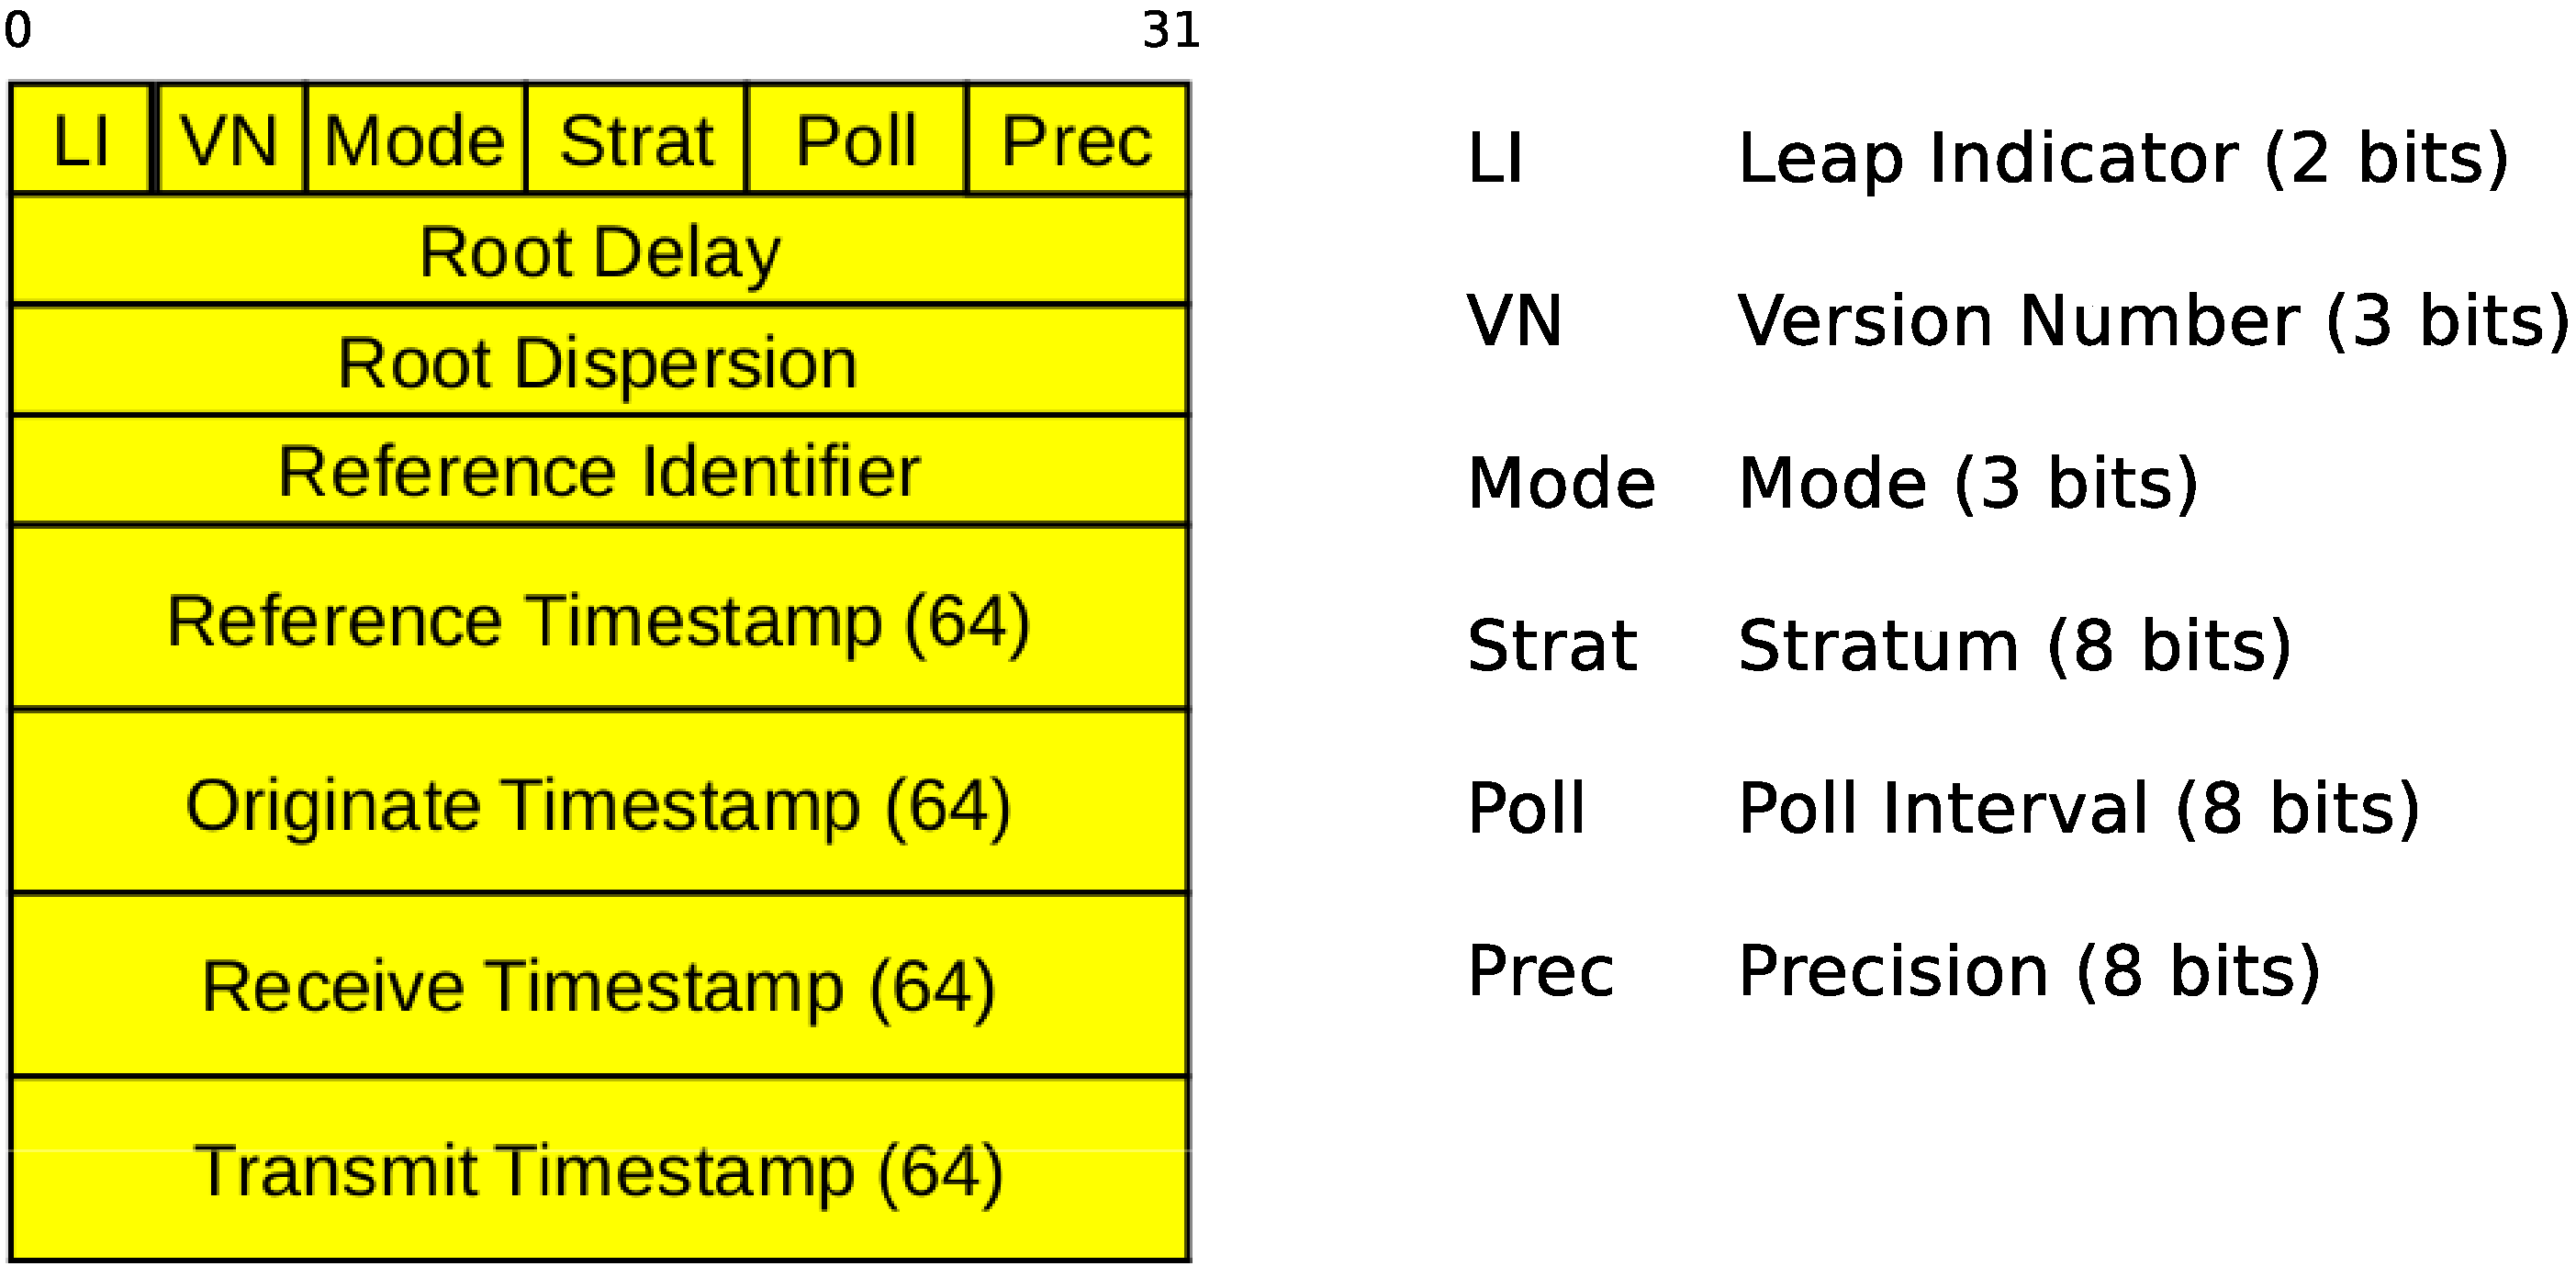
\includegraphics[width=9cm,keepaspectratio]{fig/ntp-packet.pdf}
	\caption{Basic NTP packet structure by D. Mills}
	\label{fig:ntp-packet}
	\bigskip
\end{figure}

Because Root dispersion and Root Delay fields do not need so big scope and precision,
the short 32-bit format is used for them.
Root dispersion express accumulated total dispersion from primary server
and Root Delay express accumulated roundtrip delay via primary server~\cite{ntp-arch}.


%TODO - TIMESTAMPS
There exists approx. 232-picosecond interval, henceforth ignored, every 136 years when
the 64-bit field will be zero, which by convention is interpreted as an invalid timestamp.
%TODO

Because of network latency the timestamp received will never be exactly corresponding to
the current time.
One of the main goals of NTP is to deal with the network latency~\cite{ntp-overview}.
